\documentclass[tikz]{standalone}
\begin{document}

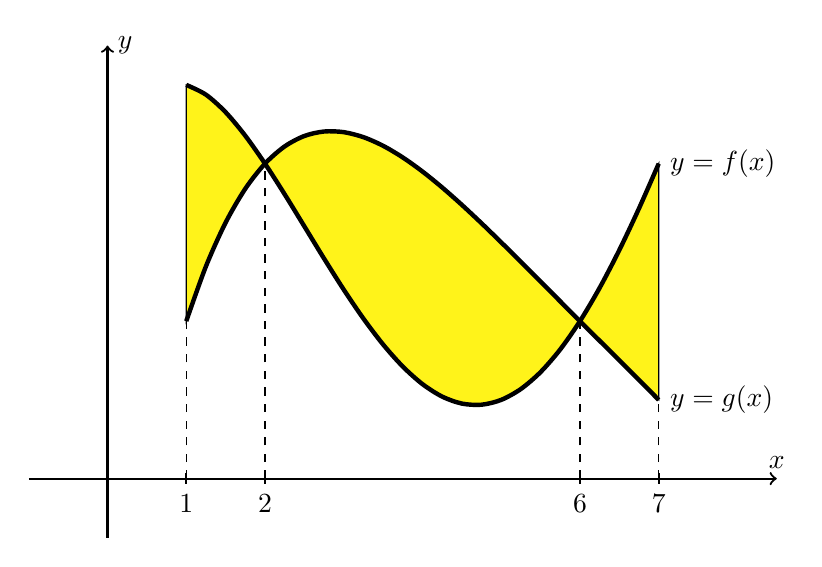
\begin{tikzpicture}

  % shade region
  \draw[smooth,fill=yellow!90] 
  plot[domain=1:7] ({\x},{-5/2 + (61*\x)/10 - (43*\x^2)/24 + \x^3/5 - \x^4/120}) --
  plot[domain=7:1] ({\x},{4 + (77*\x)/30 - (113*\x^2)/60 + \x^3/3 - \x^4/60}) -- cycle;

  % draw axes
  \draw[thick,->] (-1,0) -- (8.5,0) node[above] {$x$};
  \draw[thick,->] (0,-0.75) -- (0,5.5) node[right] {$y$};

  % draw curves
  \draw[ultra thick,domain=1:7,smooth,variable=\x,black] 
  plot ({\x},{-5/2 + (61*\x)/10 - (43*\x^2)/24 + \x^3/5 - \x^4/120}) node[right] {$y=g(x)$};
  \draw[ultra thick,domain=1:7,smooth,variable=\x,black] 
  plot ({\x},{4 + (77*\x)/30 - (113*\x^2)/60 + \x^3/3 - \x^4/60}) node[right] {$y=f(x)$};

  % tick marks
  \foreach \x in {1,2,6,7} 
    \draw [thick] (\x cm,2pt) -- (\x cm,-2pt) node[below] {$\x$};
    
  \draw[dashed] (1,0) -- (1,2);
  \draw[dashed] (2,0) -- (2,4);
  \draw[dashed] (6,0) -- (6,2.1);
  \draw[dashed] (7,0) -- (7,1);

\end{tikzpicture}
\end{document} 
